\begin{appendices}

\section{Lempel-Ziv'78 pseudocode}
From~\cite{jacquet_analytic_2015}, with $\mathcal{T}.\$$ being 
the last symbol in the tree.

\label{app:lempelziv}

\SetKw{KwProcedure}{procedure}
\SetKw{KwReturn}{return}
\begin{algorithm}[H]
 \KwProcedure \textsc{Encoding}(w)\;
 $\mathcal{T} \leftarrow$ Tree(0)\;
 $k \leftarrow 1$\;
 \While{$w\neq\text{nil}$}{
  $x\leftarrow \textmd{Read}(w)$\;
  $\mathcal{T}' \leftarrow \mathcal{T}$\;
  \While{$\mathcal{T}'.x \neq \text{nil} \& w \neq \text{nil}$}{
    $\mathcal{T}' \leftarrow \mathcal{T}'.x$\;
    $x\leftarrow\textmd{Read}(w)$\;
   }{
    \If{$\mathcal{T}'.x = \text{nil}$}
    {$\mathcal{T}'.x \leftarrow Tree(k)$}
    \Else{$\mathcal{T}'.\$ \leftarrow Tree(k)$
  }
  $k\leftarrow k+1$
 }}
 \KwReturn $\mathcal{T}$
 \caption{Building the LZ'78 parsing tree}
\end{algorithm}


\newpage
\section{Code overview}
\label{app:code1}
\begin{tabular}{ll}
    &\textbf{Link:} \url{https://github.com/gliboc/lz-compression}\\
    &{\color{gray} 2500} lines of code in \emph{Python}
\end{tabular}

\bigskip
\noindent
This code repository is able to simulate two models 
from~\cite{jacquet_average_2001} : the \emph{\bfseries Lempel-Ziv model}, 
where a sequence of $n$ symbols is generated by an information
source and compressed by a LZ'78 algorithm, as well as the 
\emph{\bfseries Markov-Independent model}, where $n$ sequences are generated 
and then sequentially given to LZ'78 to generate phrases,
the $i$th phrase being the shortest prefix of the $i$th
sequence that was not seen before as a phrase. 

\bigskip
\begin{itemize}[nosep]
    \item[] {\color{gray} markov.py } 
    \item[] \quad Markov source implementation 
    \item[] {\color{gray} parallel\_tails.py} 
    \item[] \quad Fast and parallelized generation of sequence
    for the MI model
    \item[] {\color{gray} lempelziv.py} 
    \item[] \quad Lempel-Ziv'78 algorithm implementation
    \item[] {\color{gray} neininger.py  szpan.py  eigenvalues.py  normal.py} 
    \item[] \quad Functions for computing theoretical 
    expressions of mean and variance
    \item[] {\color{gray} main.py  tails.py} 
    \item[] \quad Plots graphs for visualization
    \item[] {\color{gray} experiments.py  experiment\_tails.py} 
    \item[] \quad Managing data generated for experiments
\end{itemize}

\bigskip
This repository also contains a variety of \emph{Jupyter} notebooks,
which might provide some insight into my work method. This routine 
consisted in writing code to run numerics intertwined with exact 
expression and computations written in \LaTeX. I found it to be
quite productive in terms of getting results and writing and presenting 
them. The notebooks are not polished work but drafts.

\newpage
\section{Asymptotics on the mean $E[M_n]$}

	I also tried to normalize $M_n$ using theoretical expressions
	of the mean and variance. For the mean, the first order expression
	
	\centers{$E_n \sim \f{nh}{\log_2(n)}$}
	
	\noindent
	is, under $n\leq 10^6$, not sufficient to center the distribution. I conducted a numerical analysis
	of the difference between this expression and the empirical mean for growing 
	values of $n$. In particular, here is how their difference, in black, compares with
	different approximation functions 
	
	
	  \begin{figure}
		\centering
        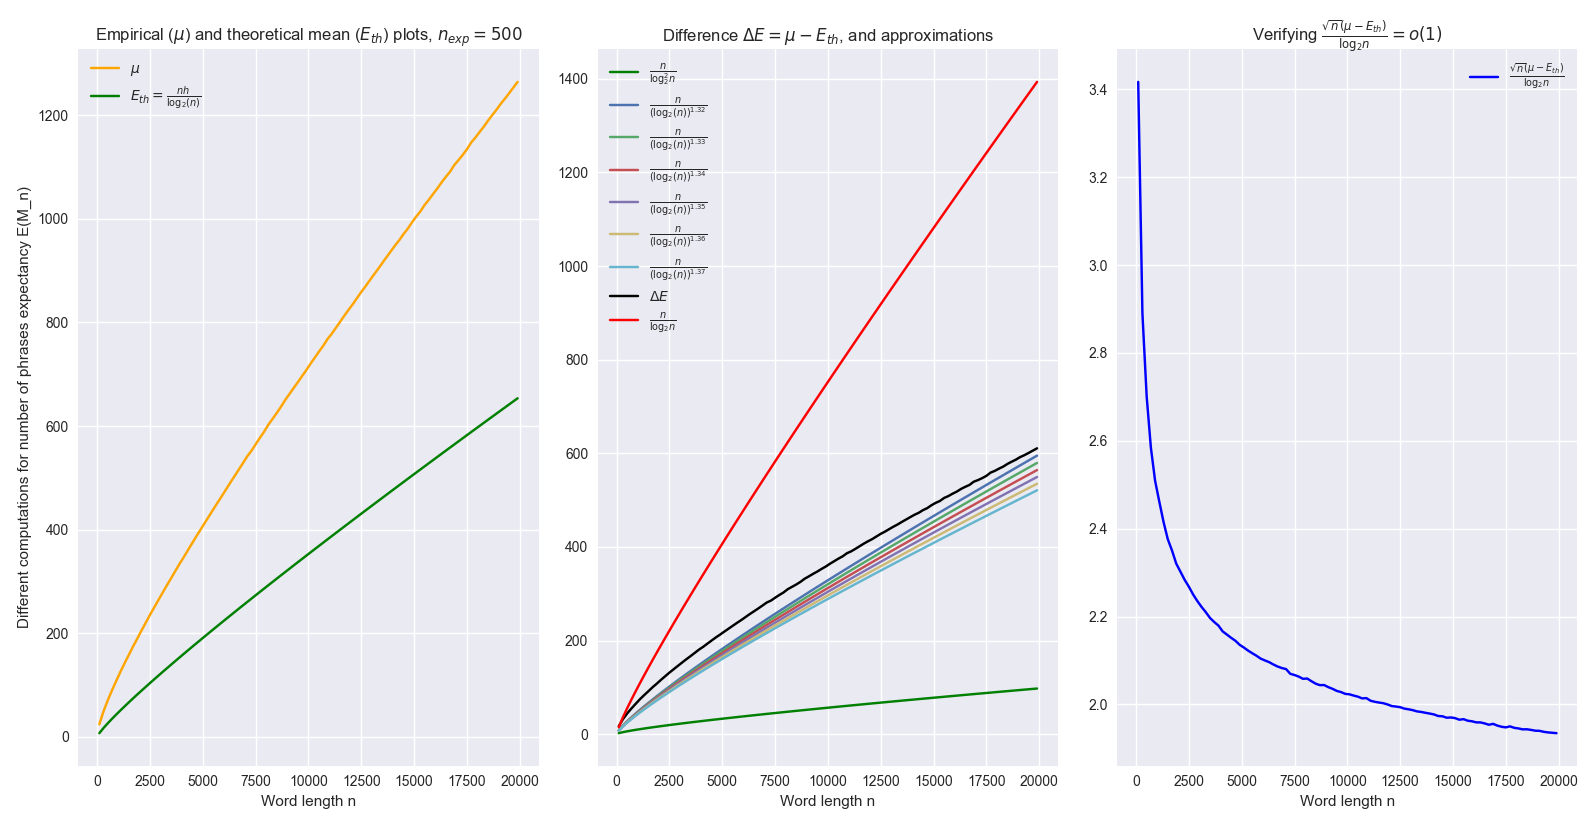
\includegraphics[width = 5cm,
        				    trim = 14cm 0 13cm 1.5cm,
								clip=true]{./figs/mean_analysis_2e4_500.png}
		\caption{Difference $\mu - \f{nh}{\log_2(n)}$ and approximation plots.}	
	  \end{figure}
	
	\noindent
	This is not troubling as it was already predicted in the formula:
	
	\centers{$E_n = 	\f{nh}{\log_2(n)} + \mathcal{O} \pa{ \f{n}{\log_2(n)} }$}


\newpage
\section{Much longer words}

These graphs are on the edge of the performance of my simulations.
Studying asymptotics numerically meant that, for too high an $n$,
I sometimes could not generate enough samples to consider a graph
accurate, even the general trend would still give me information.


\label{app:much_longer}
\begin{figure}[H]
    \centering
        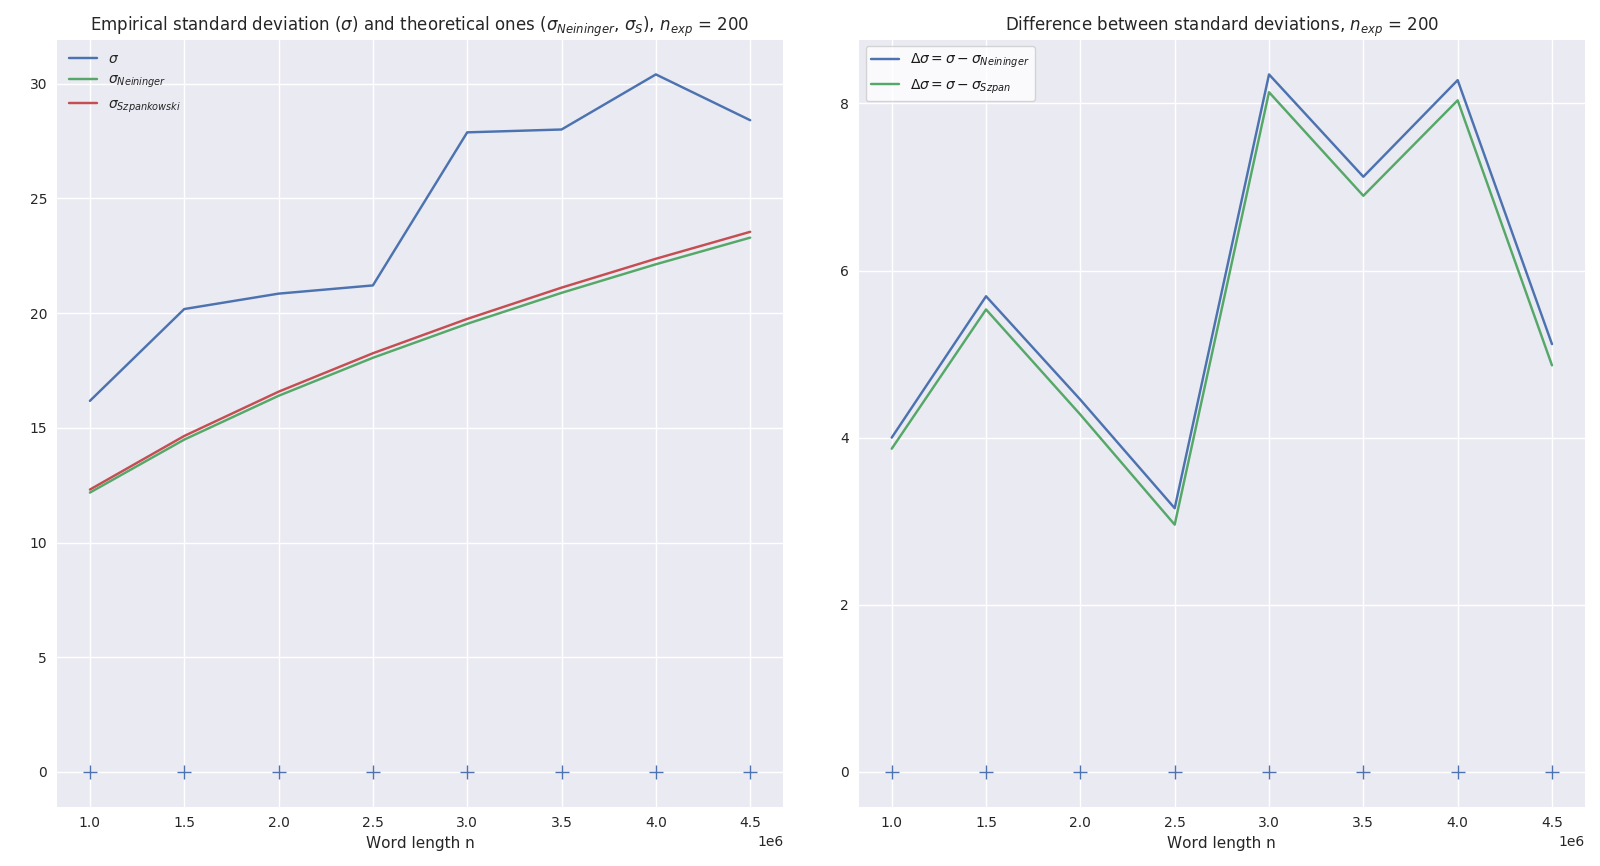
\includegraphics[width = \textwidth,
        				    trim = 0 0 0 0,
                                clip=true]{./figs/eig_fig5.png}	
    \captionsetup{justification=centering}
    \caption{Standard deviations behaviors and difference with empirical\\
            $10^6 \leq n_{\text{word}} \leq 5\cdot10^6, n_{\text{exp}}=200$}
\end{figure}

\noindent
\begin{figure}[H]
    \centering
        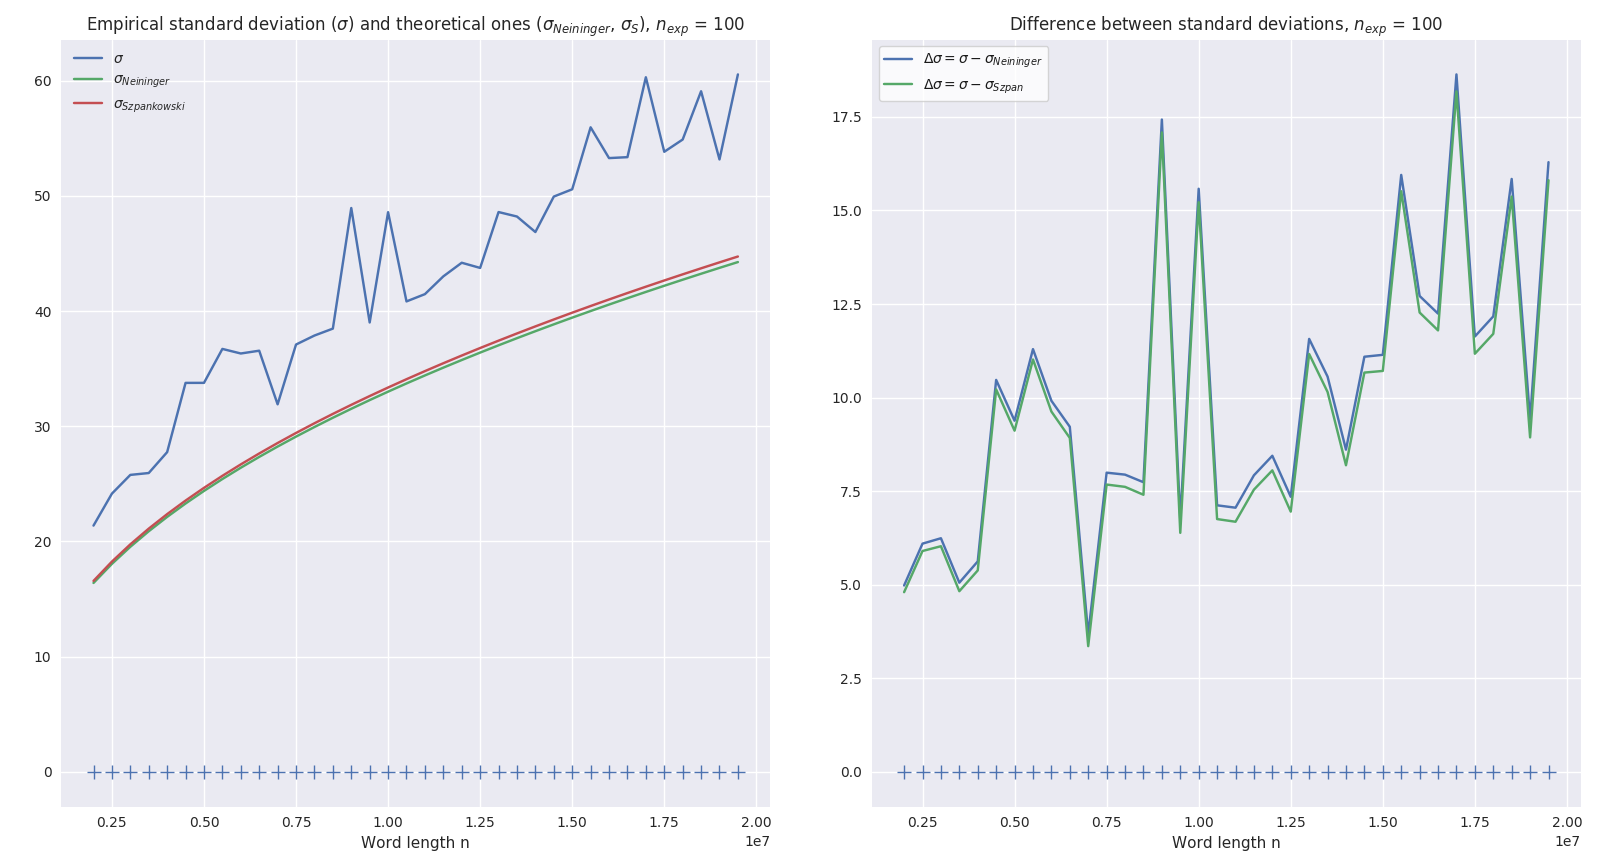
\includegraphics[width = \textwidth,
        				    trim = 0 0 0 0,
                                clip=true]{./figs/eig_fig4.png}	
    \captionsetup{justification=centering}
    \caption{Standard deviations behaviors and difference with empirical\\
    $10^7 \leq n_{\text{word}} \leq 2\cdot10^7, n_{\text{exp}}=100$}
\end{figure}

\pagebreak
\section{Another (more complicated) computation of $\ddot{\lambda}(-1)$}
\label{app:comp_lam1}
This expression gives the sames numerical results as the first one, 
but is more complex to compute for no apparent gain other than having 
yet another similar way of computing $\ddot{\lambda}(-1)$. 
Computing $\delta(s)$, a complex root of 
$\Delta(s)$, writing $\Delta$ as :

\begin{calculs}
    & \Delta 
        &=& \underbrace{p_{0 0}^{-2\Re(s)} \cos(2\ln(p_{0 0})\Im(s))}_{a_0(s)} \\[6mm]
          &&+& \underbrace{p_{1 1}^{-2\Re(s)} \cos(2\ln(p_{1 1})\Im(s))}_{a_1(s)} \\[6mm]
           &&& \underbrace{- 2 (p_{0 0}\,p_{1 1})^{-\Re(s)} \cos(\ln(p_{0 0}\,p_{1 1})\Im(s))}_{a_2(s)} \\[6mm]
           &&+&  \underbrace{4 (p_{0 1}\,p_{1 0})^{-\Re(s)} \cos(\ln(p_{0 1}\,p_{1 0})\Im(s))}_{a_3(s)} \\[6mm]
          &&+& i \Im(\Delta) 
\end{calculs}

where $\Im(\Delta) = b_0(s) + b_1(s) + b_2(s) + b_3(s)$, with each $b_i(s)$ being
the same term as $a_i(s)$ with $\cos$ replaced by $\sin$. Writing

\centers{$\Delta = \alpha(s) + i \beta(s)$}

and searching for $\delta = x(s) + i y(s)$, meaning that

\centers{$ \left\{
                \begin{array}{rl}
                    x^2 - y^2 &= \alpha \\
                    2\, x\, y &= \beta \\
                    x^2 + y^2 &= \sqrt{\alpha^2+\beta^2}
                \end{array}
            \right.
        $}
    

This yields
 
    \centers{$
        \left\{
            \begin{array}{rl}
                     x &= \pm \sqrt{\f{1}{2}(\sqrt{\alpha^2+\beta^2}+\alpha)} \\
                     y &= \pm \sqrt{\f{1}{2}(\sqrt{\alpha^2+\beta^2}-\alpha)} 
            \end{array}
        \right. 
            $}

and since $2xy = \beta$, there is $\epsilon \in \{-1,1\}$ such that
             \centers{$ \delta = \pm (x + \ir \epsilon y) $}

\leftcenters    
    {so}
    {$\lambda(s) = \f{ \poo + \pii \pm (x + \ir \epsilon y)}{2}$}

\leftcenters
    {\text{i.e.}}
    {$\ddot{{\lambda}}(-1) = \f{ p_{0 0} \ln^2(p_{0 0})
                                    + p_{1 1} \ln^2(p_{1 1})
                                    \pm (\ddot{{x}}(-1) + \ir \epsilon \ddot{{y}}(-1))}
                                  {2} $}
where we'll have to find what is $\epsilon$ and which sign to pick.

But first, computing the derivatives of $x(s) = \sqrt{f(s)} $:
    \centers{$\dot{x}(s) = \f{f'(s)}{2x(s)}$}
    \leftcenters
        {and}
        {$\ddot{{x}}(s) = \f{ f''(s) x(s) - f'(s) \cdot \f{f'(s)}{2x(s)} }
                                   { 2 x^2(s) } $}

and then computing $f(s)$ :

    \centers{$ f(s) = \f12 (\sqrt{\alpha^2+\beta^2} + \alpha) $}
    \centers{$ f'(s) = \f12 \left[ \f{ \overbrace{ \dot{\alpha}\alpha + \dot{\beta}\beta }^{ \gamma(s) } }
                                     { \underbrace{\sqrt{\alpha^2 + \beta^2}}_{\kappa(s)} }
                                    + \dot{\alpha} \right] $}

    \leftcenters{with}{$ \dot{\alpha} = \dot{a_0} + \dot{a_1} + \dot{a_2} + \dot{a_3} $}

{As for $f''(s)$, it is}
\centers
    {$ f''(s) = \f12 \left[ 
                        \f{ \dot{\gamma}(s) \kappa(s) - \gamma(s) \dot{\kappa}(s) }
                          {\kappa^2(s)} 
                        + \ddot{{\alpha}}(s) 
                    \right] $}

\leftcenters
    {with}
    {$\dot{\gamma}(s) = \ddot{{\alpha}} \alpha + {\dot{\alpha}}^2 + \ddot{{\beta}}\beta + {\dot{\beta}}^2$}

\centers
    {$ \dot{\kappa}(s) = \f{2 \alpha \dot{\alpha} + 2 \beta \dot{\beta}}
                           {2\sqrt{\alpha^2+\beta^2}}$}


Derivating according to $s$ amounts to derivating according to $\Re(s)$, so in $s=-1$ :

    \centers{$ \dot{\alpha}(-1) = -2\ln p_{0 0} a_0(-1)
                              -2\ln p_{1 1} a_1(-1)
                              -\ln q_0 a_2(-1)
                              -\ln q_1 a_3(-1) $}
and
\centers
    {$ \ddot{\alpha}(-1) = 4\ln^2 p_{0 0} a_0(-1)
                             + 4\ln^2 p_{1 1} a_1(-1)
                              +\ln^2 q_0 a_2(-1)
                              +\ln^2 q_1 a_3(-1) $}

At this point we have fully determined $\ddot{{x}}(s)$, and we realize two things:

\begin{enumerate}
    \item In $s=-1$, since $Im(-1) =0$ and because of the sinus function,
          all the $\beta$ terms, including derivatives, are equal to 0.
          This will simplify the expression for $\ddot{{x}}(-1)$.

    \item Furthermore, it also means that $\ddot{{y}}(-1) = 0$,
          so
          \encadre{ $\ddot{{\lambda}}(-1) = \f{ p_{0 0} \ln^2(p_{0 0})
                                    + p_{1 1} \ln^2(p_{1 1})
                                    + \ddot{{x}}(-1) }
                                  {2} $ }
          where the $+$ comes from the fact that $\lambda(s)$ is 
          the highest eigenvalue (and $\ddot{{x}}(-1) > 0$, so by
          continuity the expression around $s=-1$ retained the same sign)
\end{enumerate}

The final expression of $\ddot{{\lambda}}$ (as well as $\dot{\lambda}(-1))$)
can be fully expressed with $\alpha(-1), \dot{\alpha}(-1)$ and $\ddot{{\alpha}}(-1)$.
I empirically verified that $\dot{\lambda}(-1) = h$, and the final result is the same
as with the first method of computation.


% \pagebreak
% \section{Code for computing $\ddot{lambda}(-1)$}
% \label{app:comp_lam2}
% \lstinputlisting[firstline=156,lastline=206]{../src/eigenvalues.py}

\newpage
\section{Flexible parsing}
\label{app:flexible}

\subsection{Definitions}
\newtheorem{Definition}{def}

\question{Notations}

\begin{def}
Let $W$ be the random variable which outputs words of length $n$ 
(of $\Omega_n$) from a memoryless source.
\end{def}

\begin{def}
 Let $J \in \mathbb{N}^{\star}$ be a random
variable which, for every word $w$, uniformly picks the index of
one of its phrases. The joint law of $J$ with $W$ is :

\centers{$ \proba{ W=w, J=j } = 
                    \left\{ \begin{array}{l}
                        \tf{1}{M_n(w)} \quad \textmd{ if } j \leq M_n(w) \\
                        0 \qquad \qquad \textmd{ else }
                    \end{array}
                    \right. $ }
\end{def}

\begin{def}
The function defined as $g$ is a random variable that depends on $W$, therefore
we write it as $g_W$, or, during the event $\{ W=w \}$, $g_w$. 
Samely, we will study the random variable $g_W(J)$, and will
sometimes write $g_w(j)$ when both the events $[W=w]$ and $[J=j]$
occur.


\leftcenters
    {We define the random variable}
    {$B_{J, W}^k = | L_{g_W(J) - k} |$}

\noindent
and we will study the random variable
    {$ \underset{ 0 \leq k \leq g_W(J) }{ \max } 
                    \left\{ { B_{J, W}^k - k } \right\} $}

\noindent
For $J = j$, $W = w$ and $j \leq M_n(w)$, this random variable is the length of 
the $j^{\textmd{th}}$ phrase of the flexible parsing of the word $w$. We have,
accordingly,

\centers{$ D_n^{FLEX} (w) = \f{1}{M_n(w)} \Sum{j=0}{M_n(w)-1} |u_j^{FLEX}|
                          = \f{1}{M_n(w)} \Sum{j=0}{M_n(w)-1}  
                                \underset{ 0 \leq k \leq g_w(j) }{ \max } 
                                \left\{ { B_{j, w}^k - k } \right\} $}
\noindent
Precisely, $D_n^{FLEX}(w)$ is the empirical average of the lengths of the phrases
of the flexible parsing of a word $w$, whereas 
        $\underset{ 0 \leq k \leq g_w(J) }{ \max } 
        \left\{ { B_{J, w}^k - k } \right\} $,
with $J$ a random variable and $w$ fixed,
is the length of a uniformly randomly selected phrase of the flexible parsing
of $w$. 

\leftcenters   
    {Finally, we define}
    {$x_n = \f1{h} \log_2 \pa{ \f{nh}{\log_2(n)} }$}

\leftcenters
    {as well as}
    {$b_n^{\delta} = x_n + (c_3 x_n)^{\delta}$}

\leftcenters
    {and we study}
    {$ \proba{ 
        \underset{ 0 \leq k \leq g_w(J) }{ \max } 
        \left\{ { B_{J, w}^k - k } \right\}
            > b_n^{\delta} } $}

\subsection{Remarks}
\question{Corrections}

\begin{itemize}

\item The formal definition of ${D_n}^{\text{LZ}}$ in $\numero{3}$ is 
      misleading because it contradicts the previous verbal definition.
      For $w$ a word of size $n$, the formula
      \centers{$ \f{1}{M_n(w)} \Sum{j=0}{M_n(w)-1} |{u_j}^{\text{LZ}}|$}
      would rather be the empirical average length of a phrase in the Lempel-Ziv
      parsing of a word ${\barre D_n}^{\text{LZ}}$, whereas
      ${D_n}^{\text{LZ}}$ is used in the rest of the paper as the length
      of a randomly selected phrase. These two aren't equal :
      if we build a Lempel-Ziv DST from a word, then 
      ${D_n}^{\text{LZ}}$ can be seen as the depth of a random node, 
      which is different from the average path length computed 
      on all the nodes. 

\item In \emph{Remark 2}, I think the definition of $v$ and 
      $t$ should rather be 
      $ v = a_{i'} \dots a_{i} $ and
      $ t = a_{i+1} \dots a_n$. 

\item The result $\numero{14}$ should be an equality, and it is one indeed
      because of the flexible parsing algorithm. A proof by contradiction
      can show this. However, since we upperbound $g(j)$ by $\pinf$ in 
      $\numero{23}$ there might be no purpose to using $\numero{14}$ 
      instead of just $\numero{13}$. 
      % Furthermore, an equality is 
      % needed to establish result $\numero{22}$.

\item The proof around \emph{Theorem 1} has several flaws.
      The notation $X$ for a sequence depending on $n$ and not a 
      random variable is misleading. On the other hand, it should appear
      that both $g$ and $j$ are random variables, as the randomness of 
      $j$ is used in the end of the proof.
      I wrote some possible definitions \hyperlink{definitions}{here},
      and applied them to make some computations that seemed otherwise
      incorrect because of their use of randomness outside of a probability
      measure (\hyperlink{computations}{here}).

\item As for the arguments that 
      link $|L_{g(j)-k}|$ to ${D_n}^{\text{LZ}}$, I have
      indicated how I think they could be developped in 
      \hyperlink{critics}{this part.} These arguments
      are the most controversial part right now I think.

\item \emph{Theorem 2} is false as stated: we proved \emph{Theorem 1}
      using a random $j$. The randomness remains, so the quantifier
      'for any $j < M_n$' should be removed. This would be true for 
      \emph{Theorem 1} too.

\item The proof of \emph{Theorem 2} may stop at $\numero{26}$
      since we can directly prove this upperbound goes to $0$.
      This yields a tighter upperbound for \emph{Theorem 2}.
      I detailed this analysis in the 
      \hyperlink{upperbound}{last part of this report.}

\item In that same proof, the step between $\numero{25}$ and 
      $\numero{26}$ relies heavily on a result from $\pac{6}$.
      A bit more context on this result (and why it does apply here)
      would make things clearer.

\item The conclusion claims to use \emph{Cramer's} theorem to link
      \centers{$\underset{ 0 \leq k \leq g_{\scriptscriptstyle W}(J) }{ \max } 
                    \left\{ { L_{g_{\scriptscriptstyle W}(J)-k} - k } \right\}$}
      to ${D_n}^{\text{FLEX}}$, which is a sum of random variables.
      Since \emph{Cramer} applies to independent random variables and the 
      lengths of successive phrases are not independent, something must be missing 
      there.
      
\end{itemize}

\subsection{Probabilistic computation}
\hypertarget{computations}{\section{Computations}}
To prove that the definitions I introduced were useful to reason 
and write proof around the subject, I rewrote some computations which
were, in their actual form in the draft, not formally accurate though
understandable.

With these definitions, 
we can do the formal computations at the beginning 
of the proof of \emph{Theorem 1}.

By conditionning on $W$ and $J$, we obtain

\begin{calculs}
        & \proba{ \underset{ 0 \leq k \leq g_W(J) }{ \max } 
        \left\{ { B_{J, W}^k - k } \right\} > {b_n}^{\delta} }
            &=& \Sum{w \in \Omega_n}{} \Sum{j \in \mathbb{N}^{\star}}{} \,
                \proba{ \underset{ 0 \leq k \leq g_W(J) }{ \max } 
        \left\{ { B_{J, W}^k - k } \right\} > {b_n}^{\delta}, W=w, J=j } \\[5mm]
            
            &&=& \Sum{w \in \Omega_n}{} \Sum{j \in \mathbb{N}^{\star}}{} \,
                \proba{ \union{k=0}{g_w(j)} \left\{ B_{w, j}^k > k + {b_n}^{\delta} \right\} 
                            ,W=w, J=j }\\[5mm]
            
            &&\leq&
                \Sum{w \in \Omega_n}{} \Sum{j \in \mathbb{N}^{\star}}{}
                \Sum{k=0}{g_w(j)} 
                \proba{ B_{w, j}^k > k + {b_n}^{\delta}, W=w, J=j } \\[5mm]
            
            &&\leq&
                \Sum{w \in \Omega_n}{} \Sum{j \in \mathbb{N}^{\star}}{}
                \Sum{k=0}{\pinf} \,
                \proba{ B_{w, j}^k > k + {b_n}^{\delta}, W=w, J=j }
                 \\[5mm]

            &&=&
                \Sum{k=0}{\pinf}
                \Sum{w \in \Omega_n}{} \Sum{j \in \mathbb{N}^{\star}}{} \,
                \proba{ B_{w, j}^k > k + {b_n}^{\delta}, W=w, J=j }
                 \\[5mm]

            &&=&
                \Sum{k=0}{\pinf} \,
                \proba{ B_{W, J}^k > k + {b_n}^{\delta} } \\
\end{calculs}




\noindent
For all $k\in\mathbb{N}$, we may now prove that
    \centers{
        $ \proba{ B_{J, W}^k > k + {b_n}^{\delta} } 
            \leq \proba{ {D_n}^{\text{LZ}} > k + {b_n}^{\delta} } $
    }












\subsection{Proof suggestions}

\label{app:critics}
Let $k \in\mathbb{N}$.
Currently, the proof to show this stands on three arguments :

\begin{itemize}
    \item[(1)] The first is that $L_{g_W(J)-k}$ is  
          a random phrase from the Lempel-Ziv parsing of 
          a word of length $N$, where $N \leq g_W(J) \leq n$.
          In the event $\{ N = n' \}$, we consider 
          ${D_{n'}}^{\text{LZ}}$.

    \item[(2)] The second, is that $|L_{g_W(J)-k}|$ can 
          therefore be considered the same as ${D_N}^{\text{LZ}}$
          \textit{i.e} at least equal in law.

    \item[(3)] The third is that, for all $n'\leq n$, 
        ${D_n'}^{\text{LZ}} \leq {D_n}^{\text{LZ}}$.
\end{itemize}
Although they seem generally true,
there are different problems with each of these arguments :

\begin{itemize}
    \item $N$ isn't clearly established, so 
          ${D_N}^{\text{LZ}}$ isn't really known.

    \item If we can identify $N$ and, let's say,
          condition our probability with $\{ N = n' \}$, 
          it is not obvious
          that the choice of a phrase at position ${g_W(J)-k}$
          knowing $\{ N = n' \}$
          is the same as the uniform choice that operates
          when choosing a random phrase from a word of size
          $n'$, in ${D_{n'}}^{\text{LZ}}$.

    \item As for (3), this result is true on average, but 
          not in all cases. Indeed, since ${D_n}^{\text{LZ}}$
          (resp. ${D_n'}^{\text{LZ}}$) is concentrated
          around $x_n$ (resp. $x_n'$), and $x_n'$ < $x_n$
          since $n' < n$, we can show 
          that this result holds with high probability.
          To write the proof, we may condition using
          events of the type

          \centers{$\{ | {D_n}^{\text{LZ}} - x_n | \leq {k_n}^{(1)} v_n \}$}

          \leftcenters
            {and}
            {$\{ | {D_{n'}}^{\text{LZ}} - x_{n'} | \leq {k_n}^{(2)} v_{n'} \} $}
          where 
          \centers{$ v_n = \sqrt{ \log( \tf{nh}{\log(n)} ) } $}
          \noindent
          A sketch of the proof is to
          apply concentration 
          inequalities to these events 
          while picking $({k_n}^{(1)}, {k_n}^{(2)})$ such that 
            \centers{$ {k_n}^{(1)} \, v_n + {k_n}^{(2)} \, v_{n'} < x_n - x_{n'} $}
          \noindent
          and having ${k_n}^{(1)}$ and ${k_n}^{(2)}$ go to $\pinf$ for 
          $n$ going to $\pinf$ in order for the upperbound probability
          to converge to zero. 
\end{itemize}

\subsection{Upperbound proof}
\hypertarget{upperbound}{}

Finally, while working at the white board with Wojciech, he suggested 
I try a simpler proof for establishing one of the upperbounds in the 
paper goes to 0 as $n$ goes to $\pinf$. This method was, happily, 
a success - and I hope it helps their analysis going forward.
 
 This is a proof that the upperbound 
in $\numero{26}$ goes to 0. Assuming

\centersright{ $ \SUM{k=0}{\pinf} 
            \proba{ D_n^{LZ} (W) > k + b_n^{\,\delta} }
            \leq 
            A \alpha^{ {(c_3 x_n)}^{\delta - \tf12} } 
                \Sum{i=0}{\pinf} \alpha^{ \tf{ i }{ \sqrt{ c_3 x_n } } }
        $}{ \numero{26} }

\noindent We can prove directly that the upperbound term goes to 0 
for $n$ going to $\pinf$,
without resorting to another majoration.
Since $\sqrt{c_3 x_n}$ goes to infinity for $n \rightarrow \pinf$,
we can pick $n$ such that $\sqrt{c_3 x_n} > 1$. Therefore
$\alpha^{\tf{1}{\sqrt{c_3 x_n}}} < 1$ and the geometric sum gives

\centers{ $ \SUM {i=0}{\pinf}
            \alpha^{ \tf{i}{\sqrt{c_3 x_n}} } =
                  \f { 1 } 
                     { 1 - \alpha^{ \tf 1 { \sqrt{ c_3 x_n } } } } $}

\noindent It remains to prove that 
    \centers{$ \underset{n\rightarrow\pinf}{\limt} \,\,\,
                  \f { \alpha^{ {(c_3 x_n)}^{ \delta - \tf12} } } 
                     { 1 - \alpha^{ \tf 1 { \sqrt { c_3 x_n } } }} = 0
            $}

which is done by using L'Hospital's rule.
Define :
\centers
    {$ \fonction
            {f}
            { \Rplusstar }
            { \R }
            { x }
            { \alpha^{ x^{ \delta - \tf12 } } }
      \qquad \text{ and } \qquad
      \fonction
        {g}
        { \Rplusstar }
        { \R }
        { x }
        {  1 - \alpha^{ \f1{ \sqrt{x} } } } $}

\noindent Let $x \in \intoo{0}{\pinf}$. Derivating yields :

\centers{$ f'(x) = \ln \alpha \pa {\delta - \f12}
                    \, x^{\delta - \tf32}
                    \, f(x)
            \qquad \text{ and } \qquad
     g'(x) 
        =  \ln \alpha\,\, \f 1 {2x\sqrt{x}}\, \alpha ^ {\f 1 {\sqrt{x}}} $}

We proceed to show that $\f{f'(x)}{g'(x)}$ goes to 0 as $x$ goes
to $\pinf$. We have

   \centers {
        $ \f{f'(x)}{g'(x)}
             = \f { \pa{\delta - \f12}
                    \, x^{\delta - \tf32}
                    \alpha^{ x^{ \delta - \tf12 } } }
                  { \f{1}{2x\sqrt{x}} 
                        \alpha^{ \f{1}{\sqrt{x}} } }
        = 2 \pa{\delta -\f12} x^{\delta} 
            \cdot \f { \alpha^{x^{\delta-\tf12}}}
                      { \alpha^{ \f{1}{\sqrt{x}} } } $} 

Since $\alpha^{\f{1}{\sqrt{x}}} 
        \underset{x\rightarrow\pinf}{\longrightarrow} 1$, we are left to study 
        $ x^{\delta} \alpha^{x^{\delta-\tf12}}$.

 

\begin{egalites}
 Writing & x^{\delta} \alpha^{x^{\delta-\tf12}}
        & \ex{ \delta \log x + \log \alpha \cdot x^{\delta - \tf12}}
\end{egalites}

and taking the log, since $\delta > \tf12$ and $\log \alpha < 0$ we see that

\centers{$ \delta \log x + \log \alpha \cdot x^{\delta - \tf12} 
            \underset{x\rightarrow\pinf}{\longrightarrow} \minf$}

Therefore $x^{\delta} \alpha^{x^{\delta-\tf12}} \underset{x\rightarrow\pinf}{\rightarrow} 0$,
and given that $f(0) = g(0) = 0$, L'Hospital's rule applies, proving that 
$\f{f(x)}{g(x)} \underset{x\rightarrow\pinf}{\longrightarrow} 0$.






            





\end{appendices}